\documentclass[11pt,a4paper]{article}
\usepackage[T1]{fontenc}
\usepackage[utf8]{inputenc}
\usepackage{lmodern}
\usepackage{amsmath,amssymb,amsthm,mathtools,mathrsfs}
\usepackage{graphicx,float,xcolor,multicol}
\usepackage[shortlabels]{enumitem}
\usepackage[margin=27mm]{geometry}
\usepackage{microtype,needspace,placeins}
\usepackage{tikz,tikz-cd}
\usetikzlibrary{arrows.meta,calc,positioning,patterns,decorations.pathreplacing}
\usepackage[colorlinks=true,linkcolor=teal,urlcolor=teal,citecolor=teal]{hyperref}
\setlength{\parindent}{0pt}
\setlength{\parskip}{.6em}
\setcounter{secnumdepth}{0}
\allowdisplaybreaks
\raggedbottom
\providecommand{\cross}{\times}
\DeclareUnicodeCharacter{2020}{\ensuremath{\dagger}}
\DeclareMathOperator{\supp}{supp}
\DeclareMathOperator*{\esssup}{ess\,sup}
\providecommand{\chapter}{\section}
\newenvironment{tool}[2]{\subsection*{Tool #1 --- #2}}{}
\newcommand{\ToolRef}[1]{Tool #1}
\newcommand{\FigureTag}[2]{\textit{Figure #1}}
\newcommand{\Result}[1]{\subsection*{#1}}
\newcommand{\Application}[1]{\subsubsection*{Application\if\relax\detokenize{#1}\relax\else\space--- #1\fi}}
\newcommand{\ProofHeading}{\par\textit{Proof.}\space}
\newcommand{\ProofOf}[1]{\par\textit{Proof of #1.}\space}
\newcommand{\RemarkHeading}{\par\textbf{Remark.}\space}
\newcommand{\NoteHeading}{\par\textbf{Note.}\space}
\newcommand{\ExerciseHeading}{\par\textbf{Exercise.}\space}

% Rendering support only; mathematical text is in each independent post.
\usepackage{booktabs,array,longtable}
\definecolor{HandoutBlue}{HTML}{2F6690}
\definecolor{HandoutNavy}{HTML}{17365D}
\newtheorem{theorem}{Theorem}
\newtheorem{lemma}[theorem]{Lemma}
\newtheorem{proposition}[theorem]{Proposition}
\newtheorem{corollary}[theorem]{Corollary}
\newtheorem{conjecture}[theorem]{Conjecture}
\newtheorem{definition}{Definition}
\newtheorem{example}{Example}
\newtheorem{namedtoolcounter}{Tool}
\newenvironment{namedtool}[1]{\begin{namedtoolcounter}[#1]}{\end{namedtoolcounter}}
\newtheorem*{claim}{Claim}
\newtheorem*{remark}{Remark}
\newtheorem*{exercise}{Exercise}
\newtheorem*{question}{Question}
\newtheorem*{observation}{Observation}
\newcommand{\SourceChapter}[2]{\section*{#2}}
\newcommand{\Lecture}[2]{\section*{Lecture #1: #2}}
\newcommand{\unclear}[1]{\textit{[unclear: #1]}}
\newcommand{\sourcegap}{\textit{[unfinished in the source]}}
\DeclareMathOperator{\dist}{dist}
\DeclareMathOperator{\id}{id}
\DeclareMathOperator{\Hol}{Hol}
\DeclareMathOperator{\Per}{Per}
\DeclareMathOperator{\Fix}{Fix}
\DeclareMathOperator{\diam}{diam}
\DeclareMathOperator{\Var}{Var}
\DeclareMathOperator{\Leb}{Leb}
\DeclareMathOperator{\Hom}{Hom}
\DeclareMathOperator{\End}{End}
\DeclareMathOperator{\Ann}{Ann}
\DeclareMathOperator{\Spec}{Spec}
\DeclareMathOperator{\Max}{Max}
\DeclareMathOperator{\Ob}{Ob}
\DeclareMathOperator{\Tor}{Tor}
\DeclareMathOperator{\Ass}{Ass}
\DeclareMathOperator{\Mor}{Mor}
\DeclareMathOperator{\Fun}{Fun}
\DeclareMathOperator{\Nat}{Nat}
\DeclareMathOperator{\Cone}{Cone}
\DeclareMathOperator{\MCG}{MCG}
\DeclareMathOperator{\Aut}{Aut}
\DeclareMathOperator{\Deck}{Deck}
\DeclareMathOperator{\SL}{SL}
\DeclareMathOperator{\PSL}{PSL}
\DeclareMathOperator{\Area}{Area}
\DeclareMathOperator{\im}{im}
\DeclareMathOperator{\PSh}{PSh}
\newcommand{\CRing}{\mathsf{CRings}}
\newcommand{\AMod}{A\text{-}\mathsf{Mod}}
\newcommand{\Ab}{\mathsf{Ab}}
\newcommand{\Z}{\mathbb Z}
\newcommand{\Q}{\mathbb Q}
\newcommand{\R}{\mathbb R}
\newcommand{\C}{\mathbb C}
\newcommand{\N}{\mathbb N}
\newcommand{\kk}{\mathbb k}
\renewcommand{\aa}{\mathfrak a}
\newcommand{\bb}{\mathfrak b}
\newcommand{\pp}{\mathfrak p}
\newcommand{\qq}{\mathfrak q}
\newcommand{\mm}{\mathfrak m}
\newcommand{\nn}{\mathfrak n}
\newcommand{\rad}{\mathrm r}
\newcommand{\cat}[1]{\mathsf{#1}}
\setcounter{secnumdepth}{0}
\allowdisplaybreaks

\graphicspath{{figures/commutative-algebra/}}
\begin{document}
\section*{The Spectrum of a Ring}
% BLOG-CONTENT-BEGIN
\subsection{Spectrum of a ring}
Throughout, $A$ is a commutative ring.
\setcounter{definition}{16}\begin{definition}
\begin{enumerate}[label=(\roman*)]
\setcounter{enumi}{0}\item $\Spec(A):=\{\pp\mid\pp\text{ is prime in }A\}$. In particular, $\Spec(0)=\varnothing$.
\setcounter{enumi}{1}\item For an ideal $I<A$, set
\[V(I):=\{\pp\in\Spec(A)\mid I\subseteq\pp\},\qquad D(f):=A\setminus V((f))\quad(f\in A).\]
% Author check: the source writes A, not Spec(A), in the complement defining D(f).
\end{enumerate}
\end{definition}
\setcounter{theorem}{29}\begin{proposition}
For ideals $I,J<A$:
\begin{enumerate}[label=(\roman*)]
\setcounter{enumi}{0}\item $V(I)\cup V(J)=V(I\cap J)$.
\setcounter{enumi}{1}\item $\bigcap_{\lambda}V(I_{\lambda})=V(\sum_{\lambda}I_{\lambda})$.
\setcounter{enumi}{2}\item $V(A)=\varnothing$ and $V(0)=\Spec(A)$.
\end{enumerate}
\end{proposition}
\begin{proof}
(i) If $I\cap J\subseteq\pp$, then either $I\subseteq\pp$ or $J\subseteq\pp$. Clearly $V(I)\cup V(J)\subseteq V(I\cap J)$.

(ii) If $\pp\in\bigcap_{\lambda}V(I_{\lambda})$, then $I_{\lambda}\subseteq\pp$ for every $\lambda$, so $\sum_{\lambda}I_{\lambda}\subseteq\pp$. Conversely, $\pp\in V(\sum_{\lambda}I_{\lambda})$ implies $\sum_{\lambda}I_{\lambda}\subseteq\pp$, and therefore $I_{\lambda}\subseteq\pp$ for every $\lambda$.
% The last handwritten membership sign is normalized to inclusion, as in the preceding line.
\end{proof}
The proposition gives a topology on $\Spec(A)$ whose closed subsets are the $V(I)$, for ideals $I<A$. In particular, $D(f)$ is open for every $f\in A$. The sets $D(f)$ are the \emph{distinguished open sets}, and $\{D(f)\}_{f\in A}$ forms a basis for this topology, called the \emph{Zariski topology}.
% Source page 2
\setcounter{theorem}{30}\begin{lemma}
$\{\pp\}\subseteq\Spec(A)$ is closed if and only if $\pp$ is maximal.
\end{lemma}
\begin{proof}
$\{\pp\}$ is closed if and only if $\{\pp\}=V(I)$ for an ideal $I<A$. This is equivalent to $I\subseteq\pp$ and $I\nsubseteq\qq$ for prime $\qq\ne\pp$, and hence to $\pp$ being maximal.
\end{proof}
\begin{remark}
Not all points of $\Spec(A)$ are closed, so $\Spec(A)$ cannot be Hausdorff. Closed points of $\Spec(A)$ correspond to maximal ideals of $A$.
% Author check: the non-Hausdorff assertion is written without qualification in the source.
For $A=\kk[x_1,\ldots,x_n]/I$, with $\kk$ algebraically closed, Nullstellensatz gives the correspondences
\[
\begin{aligned}
\text{maximal ideals of }A
&\longleftrightarrow(x-\alpha_1,\ldots,x-\alpha_n),\quad\alpha\in\kk^n\\
&\longleftrightarrow\text{closed points of }A\\
&\longleftrightarrow\text{maximal ideals of }\kk[x_1,\ldots,x_n]\text{ containing }I\\
&\longleftrightarrow\{\alpha\in\kk^n\mid p(\alpha)=0,\ p\in I\}.
\end{aligned}
\]
% Author check: the repeated unindexed x and ``closed points of A'' follow the source.
\end{remark}
\setcounter{example}{9}\begin{example}
\begin{enumerate}[label=(\roman*)]
\setcounter{enumi}{0}\item $\Spec(\C[x])=:\mathbb A^1_{\C}$ has primes $(0)$ and $(x-a)$, $a\in\C$. Closed points correspond to $a\in\C$, $a\ne0$. The point $0$ is not closed; in fact, $\overline{\{0\}}=\mathbb A^1_{\C}$. Such points are called \emph{generic}.
% Author check: the source excludes a=0 among closed points and conflates the zero ideal with the number 0; retained.
\setcounter{enumi}{1}\item $\Spec(\Z)=\{(0),p\Z\mid p\text{ prime}\}$.
% Source page 3
\setcounter{enumi}{2}\item $\Spec(\kk[\epsilon]/(\epsilon^2))=\{(\epsilon)\}$.
\end{enumerate}
\end{example}
\subsubsection{Table of analogies}
\begin{center}
\renewcommand{\arraystretch}{1.3}
\begin{tabular}{@{}p{.30\textwidth}p{.62\textwidth}@{}}
\toprule
\textsf{Algebra}&\textsf{Geometry}\\\midrule
Ring $A$&$\Spec A$\\
Prime ideals&Points of $\Spec(A)$\\
Maximal ideals&Closed points of $\Spec(A)$\\
$a\in A$&Regular function on $\Spec(A)$: $a([\pp]):=a\pmod\pp$\\
$a\in\pp$&Functions that vanish at $[\pp]$\\
$V(I)$&Vanishing set of $I$\\
$D(f)$&Nonvanishing domain of $f$\\\bottomrule
\end{tabular}
\end{center}
\setcounter{example}{10}\begin{example}[More examples]
\begin{enumerate}[label=(\roman*)]
\setcounter{enumi}{0}\item In $\Spec(\kk[\epsilon]/(\epsilon^2))$, $\epsilon([(\epsilon)])=0$, but $\epsilon\ne0$. Thus $f(x)=0$ for every $x\in\Spec A$ does not imply $f\equiv0$.
\setcounter{enumi}{1}\item $\Spec(\R[x])=\{(0),(x-a),(x^2+ax+b)\}$. Pictorially, it looks like a folding of the complex plane.
% Author check: the condition of irreducibility on the quadratic is absent in the source.
\begin{figure}[H]\centering
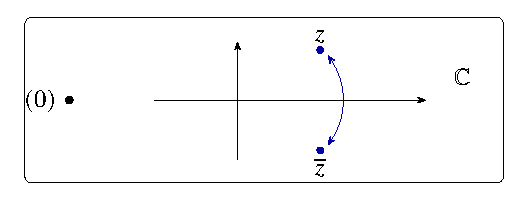
\includegraphics[width=.68\textwidth]{ca6-fig-01.pdf}
\FigureTag{CA6.1}{fig:ca-6-01}
\end{figure}
\end{enumerate}
\end{example}
% Source page 4
Let $\varphi:A\to B$ be a ring homomorphism. It induces $f=\Spec(\varphi):\Spec(B)\to\Spec(A)$.
\begin{claim}
$f$ is continuous, so $\Spec$ is a functor.
\end{claim}
\begin{proof}
For $V(I)$ in $\Spec(A)$,
\[
\begin{aligned}
f^{-1}(V(I))
&=\{\qq\in\Spec(B)\mid\varphi^{-1}(\qq)\in V(I)\}\\
&=\{\qq\in\Spec(B)\mid\qq\in\varphi(V(I))\}\\
&=\{\qq\in\Spec(B)\mid\qq\in V(I^e)\}
=V(I^e).
\end{aligned}
\]
% Author check: the middle expression phi(V(I)) is retained as written.
\end{proof}
% BLOG-CONTENT-END
\end{document}
